\documentclass[color=usenames,dvipsnames]{beamer}

\mode<presentation> {

\usetheme{Madrid}

\usepackage{tabularx}

\usepackage{multirow}

\usepackage{tikz}
\usetikzlibrary{shapes.geometric, arrows}

\usepackage{hyperref}
\hypersetup{%
	colorlinks=true,% hyperlinks will be coloured
	allcolors=ERC7
}

\definecolor{ERC1}{HTML}{C72321}
\definecolor{ERC2}{HTML}{861719}
\definecolor{ERC3}{HTML}{FBD7A9}
\definecolor{ERC4}{HTML}{BA9F7C}
\definecolor{ERC5}{HTML}{7A6952}
\definecolor{ERC6}{HTML}{6E9B9E}
\definecolor{ERC7}{HTML}{0D8085}
\definecolor{ERC8}{HTML}{19484C}
\definecolor{ERC9}{HTML}{F0C320}
\definecolor{ERC10}{HTML}{AF8F19}


\tikzstyle{startstop} = [rectangle, rounded corners, minimum width=3cm, minimum height=1cm,text centered, draw=black, fill=ERC8]
\tikzstyle{io} = [trapezium, trapezium left angle=70, trapezium right angle=110, minimum width=3cm, minimum height=1cm, text centered, draw=black, fill=ERC7]
\tikzstyle{process} = [rectangle, minimum width=3cm, minimum height=1cm, text centered, draw=black, fill=ERC9]
\tikzstyle{decision} = [diamond, minimum width=3cm, minimum height=1cm, text centered, draw=black, fill=ERC10]
\tikzstyle{arrow} = [thick,->,>=stealth]


\setbeamercolor{palette primary}{bg=ERC1,fg=white}
\setbeamercolor{palette secondary}{bg=ERC2,fg=white}
\setbeamercolor{palette tertiary}{bg=ERC3,fg=white}
\setbeamercolor{palette quaternary}{bg=ERC4,fg=white}
\setbeamercolor{structure}{fg=ERC5} % itemize, enumerate, etc
\setbeamercolor{section in toc}{fg=ERC6} % TOC sections

%gets rid of bottom navigation bars
\setbeamertemplate{footline}[frame number]{}

%gets rid of bottom navigation symbols
\setbeamertemplate{navigation symbols}{}

%gets rid of footer
%will override 'frame number' instruction above
%comment out to revert to previous/default definitions
\setbeamertemplate{footline}{}

% Override palette coloring with secondary
%\setbeamercolor{subsection in head/foot}{bg=UBCgrey,fg=white}


%\usecolortheme{lily}
\useoutertheme{infolines}

}


\usepackage{booktabs} 
\usepackage{tikz}


% Thin fonts
\usepackage{cmbright}
\usepackage[T1]{fontenc}

\definecolor{dark_grey}{gray}{0.5}
%\setbeamercolor{normal text}{fg=dark_grey,bg=white}
\setbeamertemplate{navigation symbols}{}

%\setbeamercolor*{palette primary}{fg=gray!100,bg=gray!10}
%\setbeamercolor*{palette quaternary}{fg=gray!100,bg=gray!10}
%\setbeamercolor*{palette secondary}{fg=gray!100,bg=gray!20}
%\setbeamercolor*{palette tertiary}{fg=gray!100,bg=gray!10}
%\setbeamercolor*{navigation symbols}{fg=white,bg=white}
\usefonttheme{default}


\setbeamertemplate{blocks}[rounded][shadow=false]
%\setbeamercolor{block title}{bg=gray!10}
%\setbeamercolor{block body}{fg=gray,bg=gray!10}
%\setbeamercolor{frametitle}{fg=}

\setbeamertemplate{frametitle}[default][center]

\setbeamertemplate{itemize items}[default]
\setbeamertemplate{enumerate items}[default]

\newcommand{\F}{\mathbb{F}}

\setbeamertemplate{title page}[default][colsep=-4bp,rounded=true]

\title[Workshop - Machine Learning]{ Don't believe the hype? A hands-on introduction to machine-learning in Python - Part III}
\subtitle{Open Workshops on Computer Based Systems Modelling}

\author{Johannes Schmidt, Johann Baumgartner}
\institute{Institute for Sustainable Economic Development, BOKU, Vienna}
\date{7.05.2019}

\begin{document}

{
\usebackgroundtemplate{
 \begin{picture}(320,315)
 \hspace{6.9cm}
   
\includegraphics[width=0.7\linewidth]{../figures/refuel_logo_with_text.png}
 \end{picture}
 }


\begin{frame}

\maketitle



\end{frame}
}

\begin{frame}{Contents}
\begin{itemize}
	\item A word on the blackbox
	\item Pattern recognition with neural networks: some work in progress
	\item Q-Learning
\end{itemize}
\end{frame}

% Uncomment these lines for an automatically generated outline.
%\begin{frame}{Outline}
%  \tableofcontents
%\end{frame}
%\subsection{Mathematics}

\begin{frame}{A word on the blackbox}
\begin{itemize}
	\item \href{https://christophm.github.io/interpretable-ml-book/pdp.html}{Partial dependence plot}: Average effect of one variable on output, over complete parameter space. Shows functional relationship between input and output. Assumption: inputs are all uncorrelated.
	\item Other methods are available (e.g. Accumulated Local Effects plot, Individual Conditional Expectation)  
	\item \href{http://lstm.seas.harvard.edu/}{LSTM-Vis}: visualize hidden states of LSTMs. Interesting to understand, what the hidden states may represent. See also \href{https://arxiv.org/pdf/1903.07903.pdf}{this} for an example of what hidden states represent in hydrology.
\end{itemize}
\end{frame}

\begin{frame}{Pattern recognition with neural networks: work in progress}
\begin{itemize}
	\item Validating the Global Power Plant Database with satellite fotos...
	\item Work in progress. Results not extremely promising. Recommendations very much welcome.
\end{itemize}
\end{frame}


\begin{frame}{Global Power Plant Database: Need for Validation}
\center{
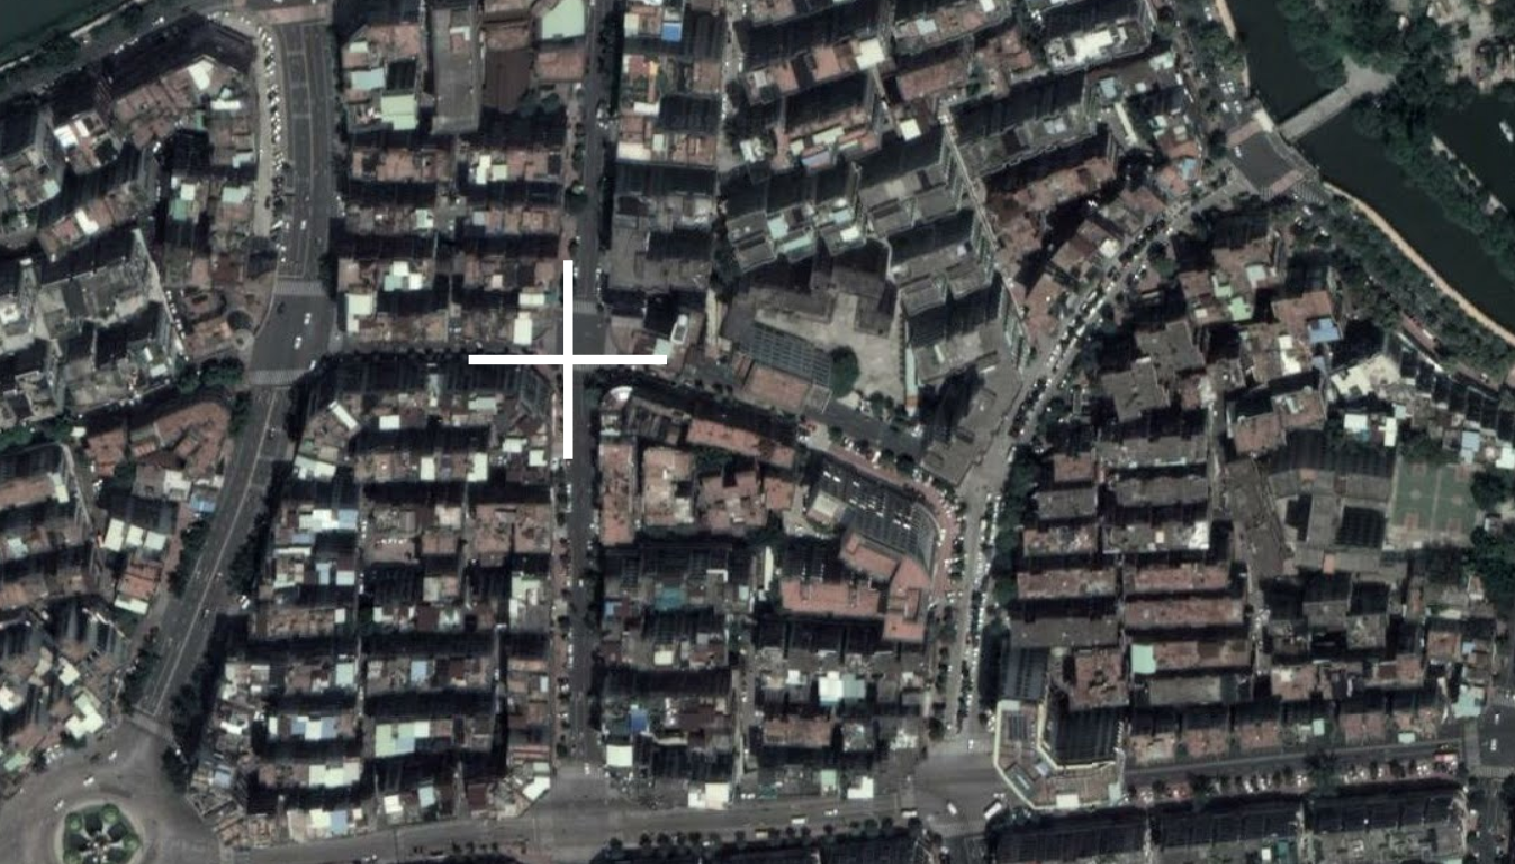
\includegraphics[width=\linewidth]{../figures/wrong_location.png}
}

\end{frame}


\begin{frame}

\frametitle{Satellite data for validation}


\framesubtitle{Sentinel-2 (10 meter resolution), free}
	\center{
	
\includegraphics[width=\linewidth]{../figures/sentinel-2.png}
}

\end{frame}

\begin{frame}
\frametitle{Satellite data for validation }
\framesubtitle{WorldView-4, Quickbird (0.31-0.65 meter resolution) used by e.g. Google Maps}

\center{
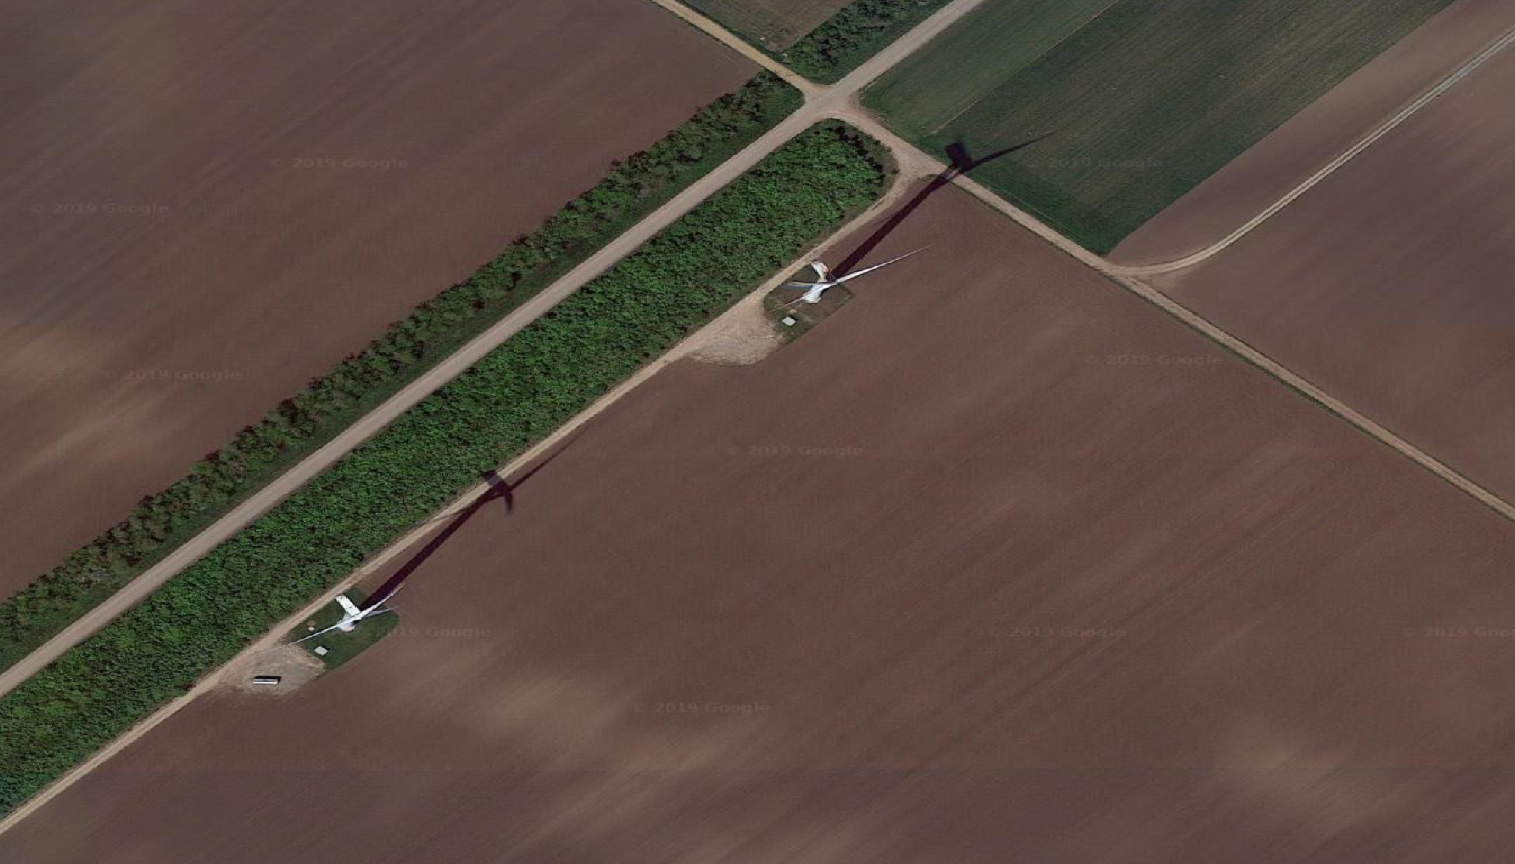
\includegraphics[width=\linewidth]{../figures/googlemaps.png}
}

\end{frame}

\begin{frame}
\frametitle{Approach}

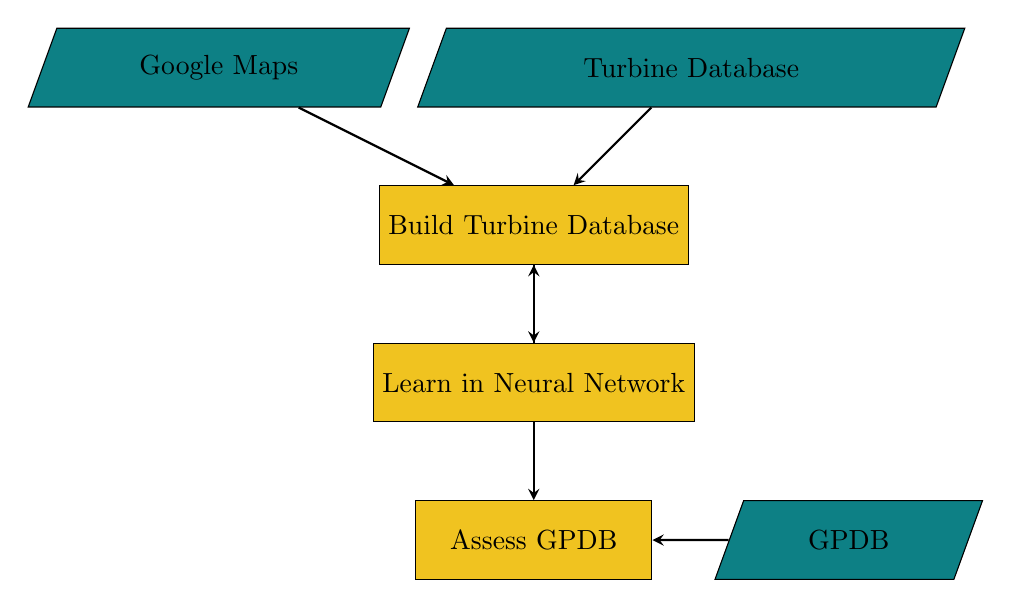
\begin{tikzpicture}[node distance=2cm]

%\node (Start) [startstop] {Start};

\node (in1) [io] {Google Maps};
\node (in2) [io, right of=in1, xshift=4cm] {Turbine Database};

\node (pro1) [process, below of=in1, xshift=4cm] {Build Turbine Database};


\node (pro2) [process, below of=pro1] {Learn in Neural Network};
\node (pro3) [process, below of=pro2] {Assess GPDB};
\node (in3)  [io, right of=pro3, xshift=2cm] {GPDB};


\draw [arrow] (in1) -- (pro1);
\draw [arrow] (in2) -- (pro1);

\draw [arrow] (pro1) -- (pro2);
\draw [arrow] (pro2) -- (pro1);
\draw [arrow] (pro2) -- (pro3);
\draw [arrow] (in3) -- (pro3);

\end{tikzpicture}

\end{frame}


\begin{frame}
\frametitle{Software}

\begin{itemize}
 \item Downloading of data from google maps: R (RGdal, tidyverse, raster)
 \item Machine Learning: Python (keras, scikit-image, gdal)
 \item Mixing R and Python: not a brilliant idea. Just lazy.
 
 
\end{itemize}

\end{frame}



\begin{frame}
\frametitle{Create Sample Database}
\framesubtitle{Manual quality control}

\center{
Positives
}

\begin{table}[ht]
\centering
\begin{tabular}{cccc}
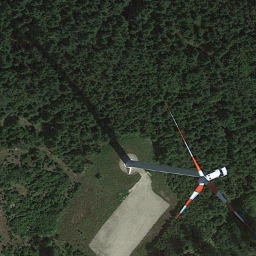
\includegraphics[width=0.2\linewidth]{../figures/wt_at_1.png}&
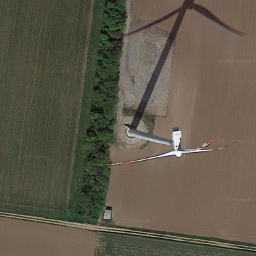
\includegraphics[width=0.2\linewidth]{../figures/wt_at_2.png}&
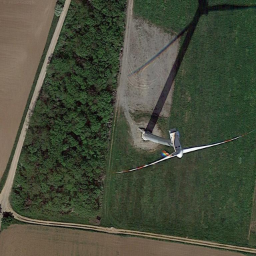
\includegraphics[width=0.2\linewidth]{../figures/wt_at_3.png}&
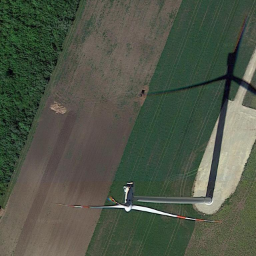
\includegraphics[width=0.2\linewidth]{../figures/wt_at_4.png}\\
\end{tabular}
\end{table}

\begin{center}
Negatives
\end{center}

\begin{table}[ht]
\centering
\begin{tabular}{cccc}
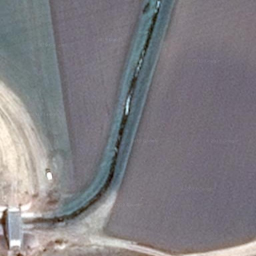
\includegraphics[width=0.2\linewidth]{../figures/no_wt_at_1.png}&
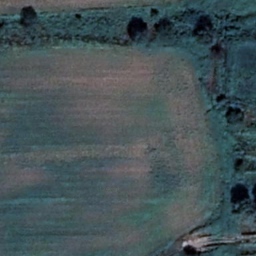
\includegraphics[width=0.2\linewidth]{../figures/no_wt_at_2.png}&
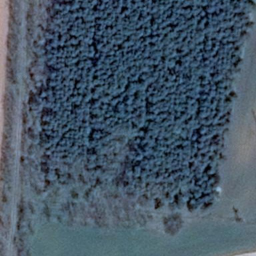
\includegraphics[width=0.2\linewidth]{../figures/no_wt_at_3.png}&
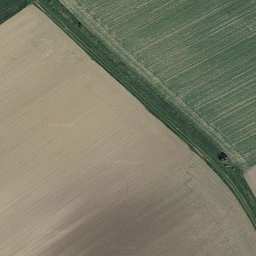
\includegraphics[width=0.2\linewidth]{../figures/no_wt_at_4.png}\\
\end{tabular}
\end{table}






\end{frame}


\begin{frame}
\frametitle{Learn with Convolutional layers}

\begin{center}
	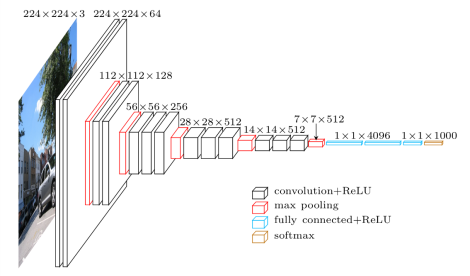
\includegraphics[width=0.8\linewidth]{../figures/vgg16.png}
\end{center}

\end{frame}

\begin{frame}
\frametitle{Layered feature learning}

\begin{figure}
	\centering
	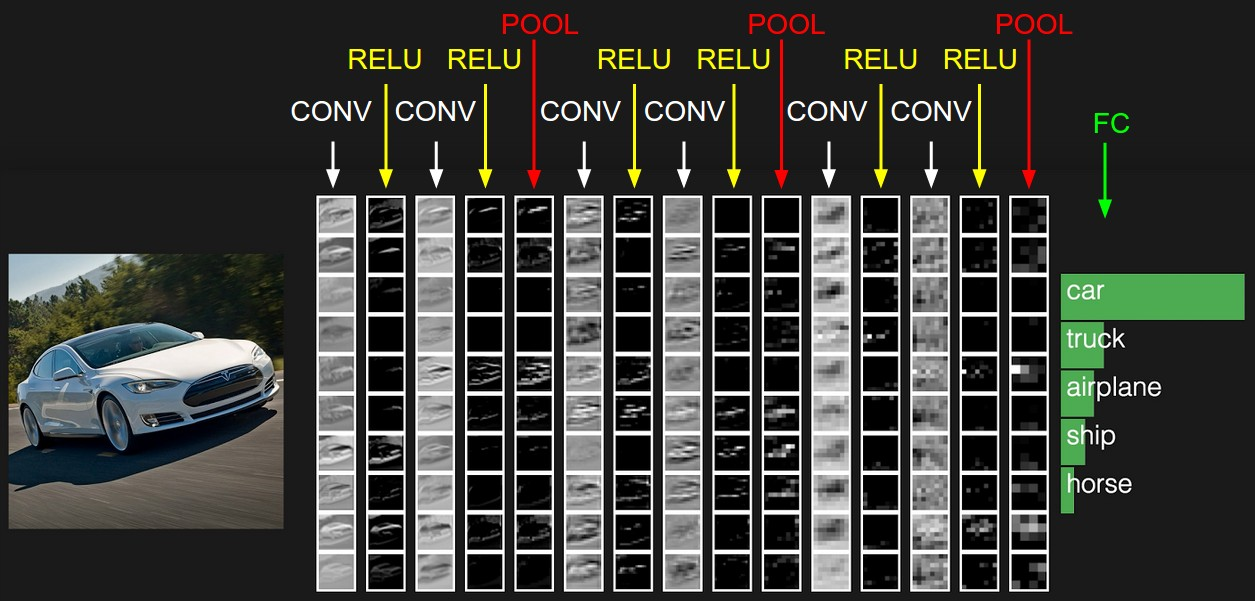
\includegraphics[width=0.8\linewidth]{../figures/convnet.jpeg}
	\caption{Taken from \href{http://cs231n.github.io/convolutional-networks/}{here}}
\end{figure}
\end{frame}

\begin{frame}
\frametitle{\href{https://ujjwalkarn.me/2016/08/11/intuitive-explanation-convnets/}{Terminology}}
\begin{itemize}
	\item Convolution operation
	\item Filter
	\item Depth
	\item Stride
	\item Zero padding (wide and narrow convolution)
\end{itemize}
\end{frame}

\begin{frame}
\frametitle{Pooling}
\begin{itemize}
	\item Makes input representations (feature dimension) smaller and more manageable
	\item Reduces the number of parameters and computations in the network controlling overfitting
	\item Makes the network invariant to small transformations, distortions and translations in the input image
	\item Helps us arriving at an almost scale invariant representation of our image (the exact term is “equivariant”)
	\item taken from \href{https://ujjwalkarn.me/2016/08/11/intuitive-explanation-convnets/}{here}
	
\end{itemize}


\end{frame}

\begin{frame}
\frametitle{Some hints}
\begin{itemize}
	\item Compile high quality training set
	\item Do not overfit!	
	\item Use pretrained networks to speed up learning process. Keras models can be found \href{https://keras.io/applications/}{here}
	\item Unfreeze last layers to learn your specific task, fixing the lower layers which extract basic features
	
\end{itemize}
\end{frame}

\begin{frame}
\frametitle{Results Learning}
\framesubtitle{Quality Measures}
\begin{centering}
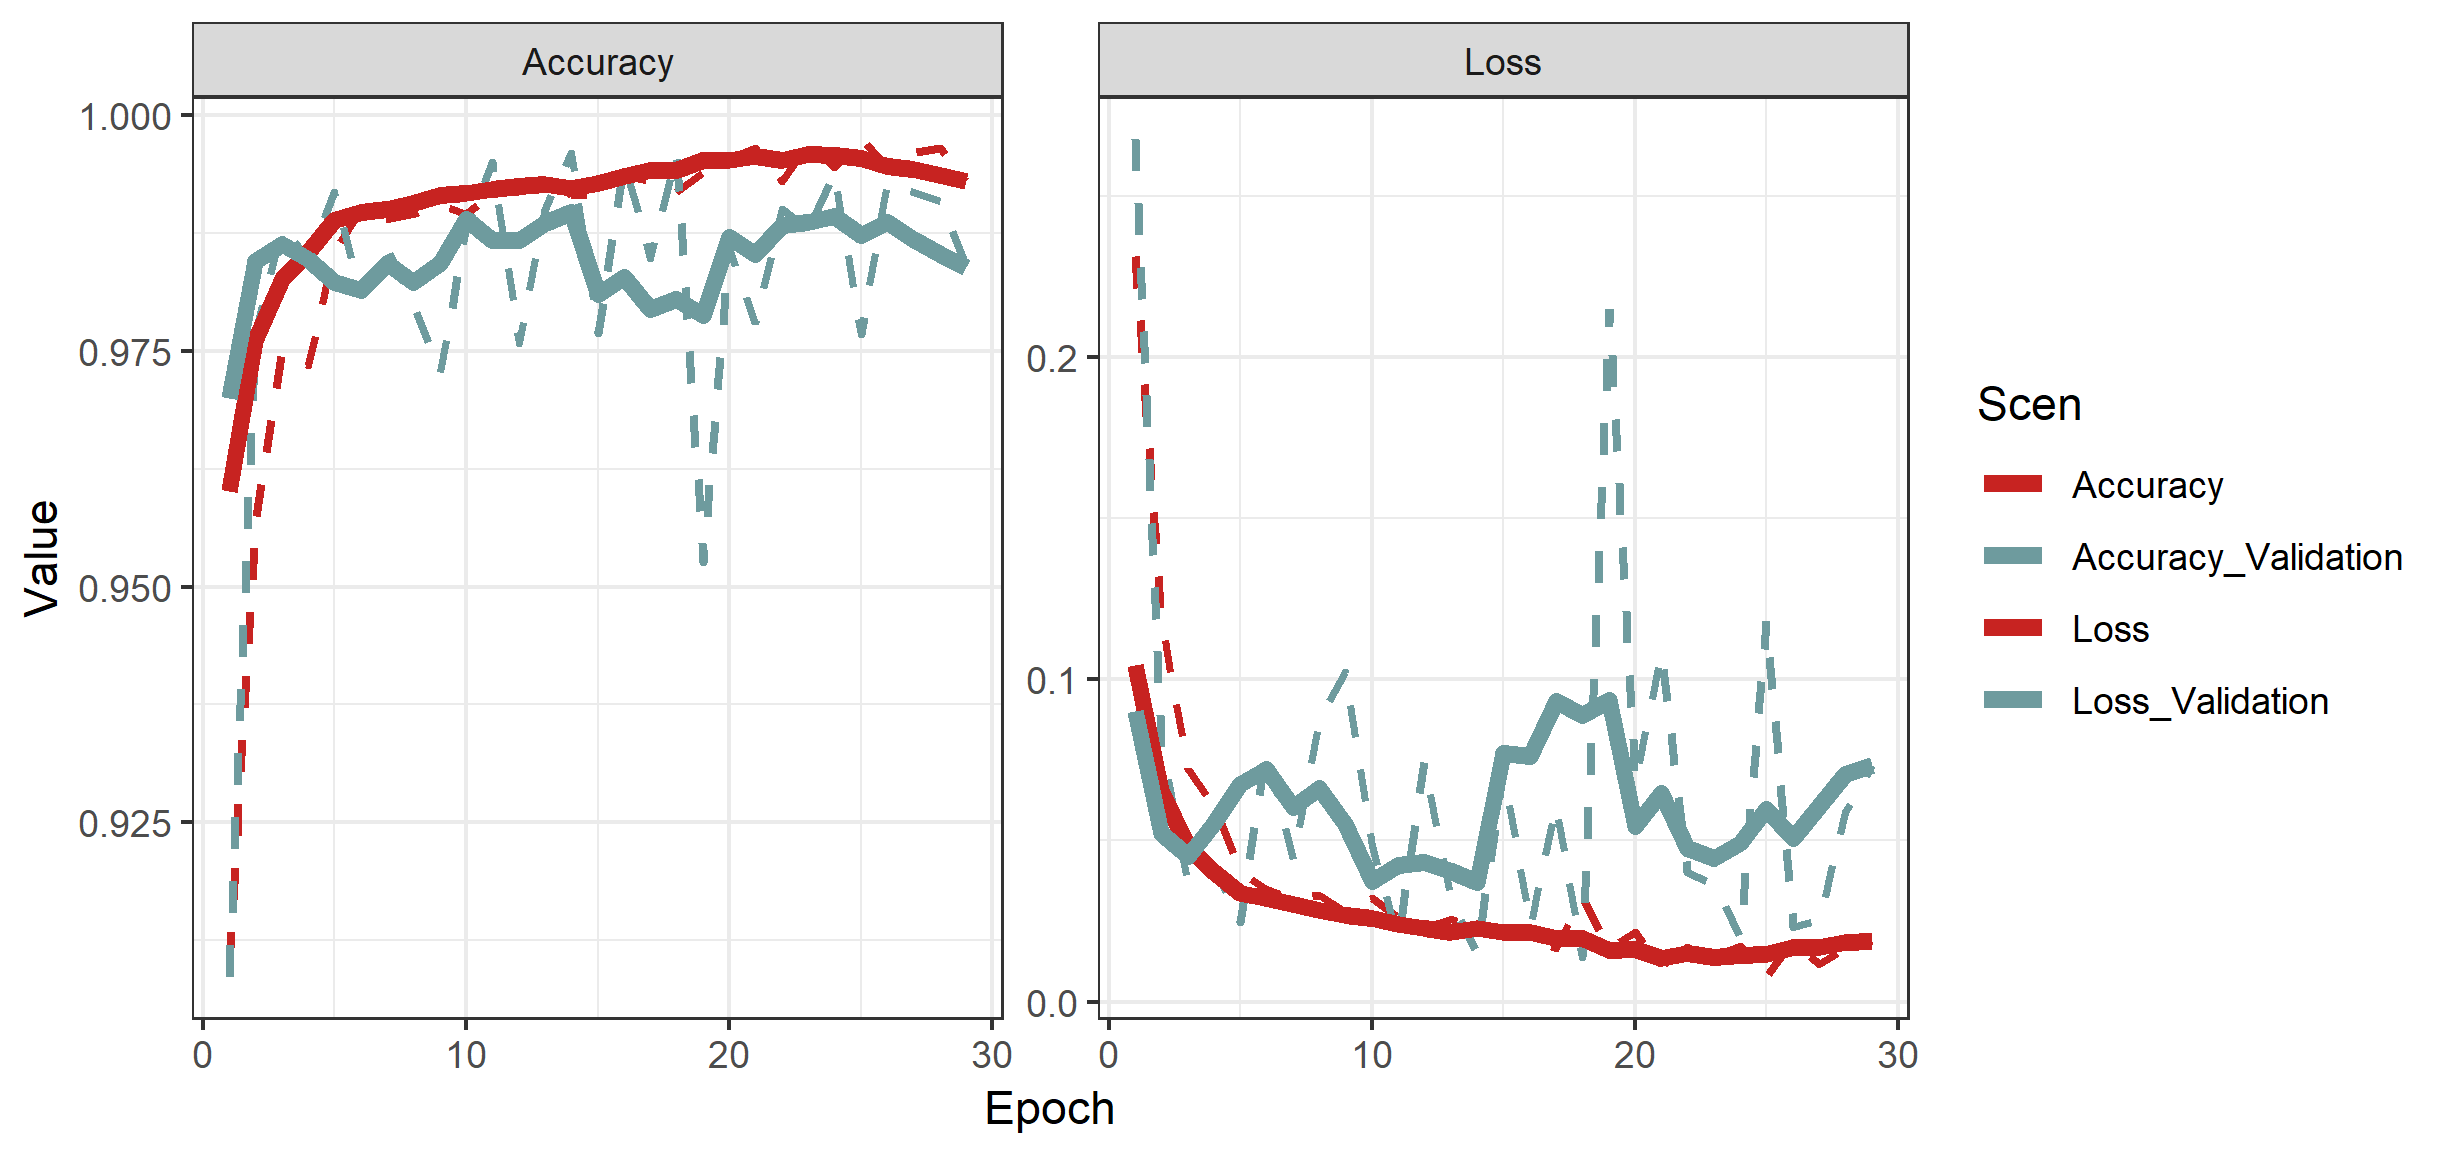
\includegraphics[width=\linewidth]{../figures/accuracy_loss.png}
\end{centering}


\begin{centering}
\begin{table}[ht]
\centering
\begin{tabular}{cc}

\tiny{
$Accuracy=\frac{Number\ of\ Correct\ Predictions}{Number\ of\ Total\ Predictions}$
} 

&
\tiny{
$Loss=-1\frac{1}{N}\sum_{i=1}{N}y_ilog(p(y_i))+(1-y_i)log(1-p(y_i))$
}

\\


\end{tabular}
\end{table}
\end{centering}

\end{frame}



\begin{frame}
\frametitle{Results Learning}
\framesubtitle{Class Activation Map}

% READ THIS: https://jacobgil.github.io/deeplearning/class-activation-maps
% makes sense for the handmade network and should make sense for the vgg16 one.

%\begin{centering}

%\begin{table}[ht]
%\centering
%\begin{tabular}{cc}

%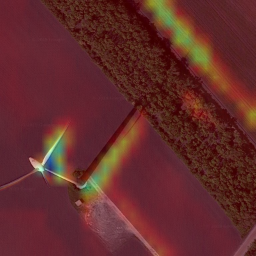
\includegraphics[width=0.4\linewidth]{../figures/heatmap_turbine.png}&
%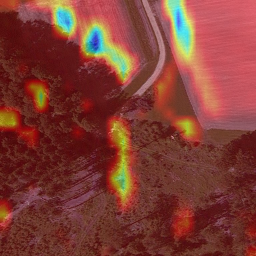
\includegraphics[width=0.4\linewidth]{../figures/heatmap_no_turbine.png}\\
%\small {Probability of being wind turbine 0.999} &
%\small {Probability of being wind turbine 0.001} \\

%\end{tabular}
%\end{table}


%\end{centering}

see notebook

\end{frame}




\begin{frame}
\frametitle{Searching wind turbines}
\framesubtitle{Create grid and check image by image}

\center{

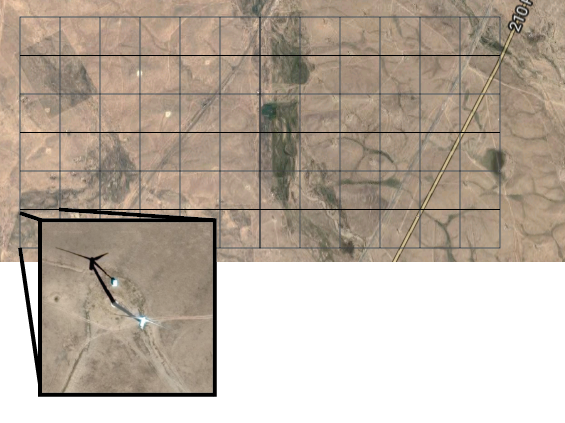
\includegraphics[width=0.8\linewidth]{../figures/grid_search.png}
}

\end{frame}



\begin{frame}
\frametitle{Application}
\framesubtitle{French Wind Parks}

\textbf{France}: 10 parks assessed. 

\begin{table}[]
	\begin{tabularx}{\textwidth}{XXXX}
	
		Turbines correctly identified  &Non-Turbines correctly identified  &Turbines wrongly identified  &Non-Turbines wrongly identified  \\
			\hline
		6  &3429  &5  &8  \\
	\end{tabularx}
\end{table}

\end{frame}

\begin{frame}
\frametitle{Discussion}
\begin{itemize}
\item Beware: Shaky legal conditions. Also, date of satellite photos unknown.
 \item Runtime prohibitive on desktop computers. For a full global check would need cluster computing with high bandwidth (but see shaky legal conditions...) 
 \item Improve classification: need for more negatives which are similiar to positives? How could we derive those? (Currently random sampling of negatives, therefore tiles do not contain a lot of cities or roads...)
\end{itemize}

\end{frame}




\begin{frame}
\frametitle{Conclusions}
\begin{itemize}
 \item Full validation of GPDB due to missing temporal information not fully possible. 
 \item Current best commercial satellite data allows identification of single turbines with good accuracy by using machine learning approaches
 \item Research limited by Data availability. Public domain data is low resolution (i.e. Sentinel-2) or small spatial domain (free ortho-photos, like basemmap.at).
\end{itemize}

\end{frame}

\begin{frame}
\frametitle{And now for something completely different...}


\end{frame}

\begin{frame}
\frametitle{Contents}
\begin{itemize}
	\item The Q-learning algorithm
	\item A very simple example calculated by hand
	\item A simple example in python
\end{itemize}

\end{frame}

\begin{frame}{Some examples}

\begin{itemize}
	\item \href{https://www.youtube.com/watch?v=W_gxLKSsSIE}{Pan flipping robot}
	\item \href{https://youtu.be/rOL6QJdAlm8?t=103}{{The moment alphaGo wins against Lee Sedol}}
	\item Automatic recommendation systems
\end{itemize}

\end{frame}


\begin{frame}{The Q-learning algorithm in a nutshell}
\framesubtitle{Which action to pick?}
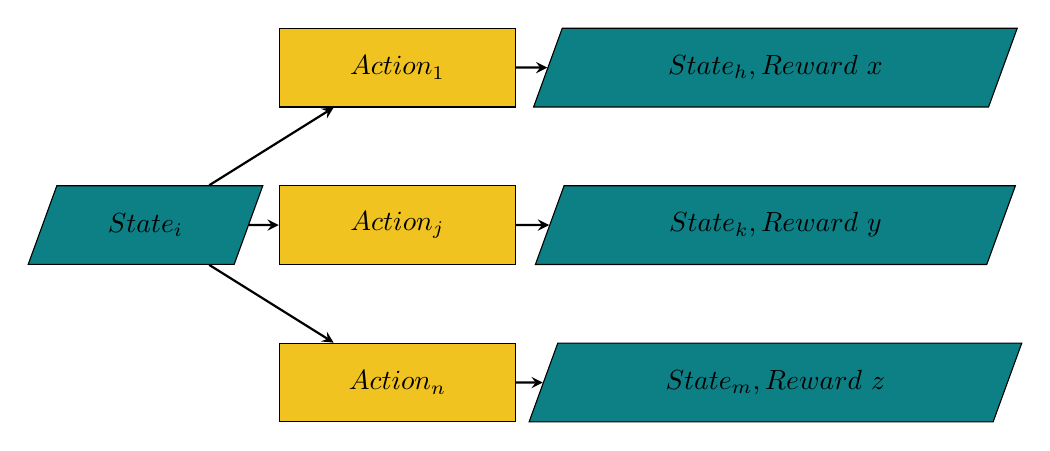
\begin{tikzpicture}[node distance=2cm]

%\node (Start) [startstop] {Start};

\node (si) [io] {$State_i$};

\node (a1) [process, right of=si, xshift=1.2cm, yshift=2cm] {$Action_1$};
\node (aj) [process, right of=si, xshift=1.2cm] {$Action_j$};
\node (an) [process, right of=si, xshift=1.2cm, yshift=-2cm] {$Action_n$};

\node (sip1) [io, right of=a1, xshift=2.8cm] {$State_{h}, Reward\ x$};
\node (sip2) [io, right of=aj, xshift=2.8cm] {$State_{k}, Reward\ y$};
\node (sip3) [io, right of=an, xshift=2.8cm] {$State_{m}, Reward\ z$};



\draw [arrow] (si) -- (a1);
\draw [arrow] (si) -- (aj);
\draw [arrow] (si) -- (an);

\draw [arrow] (a1) -- (sip1);
\draw [arrow] (aj) -- (sip2);
\draw [arrow] (an) -- (sip3);

\end{tikzpicture}
\end{frame}


\begin{frame}{The Q-Table}
\framesubtitle{The Q-Table is updated in a learning by doing approach}

Q-Updating rule introduced 1989 by Watson. Updates Q-Table according to current rewards and expected future rewards\\

$q^{new}(s_t,a_t)=(1-\alpha)q(s_t,a_t) + \alpha (r_t + \gamma \max\limits_{a} q(s_{t+1},a))$\\

$\alpha$ is learning rate, $\gamma$ is discount rate\\
$r_t$ is reward, $s_t$ is state, $a_t$ is action\\

\begin{table}
\begin{tabular}{lllll}
\multicolumn{4}{c}{Actions}\\
\multirow{4}{*}{States}		& $q_{s_1,a_1}$ & $q_{s_1,a_2}$ & $q_{s_1,a_3}$  & $q_{s_1,a_4}$\\
& $q_{s_2,a_1}$ & $q_{s_2,a_2}$ & $q_{s_2,a_3}$  & $q_{s_2,a_4}$\\
& $q_{s_3,a_1}$ & $q_{s_3,a_2}$ & $q_{s_3,a_3}$  & $q_{s_3,a_4}$\\
& $q_{s_4,a_1}$ & $q_{s_4,a_2}$ & $q_{s_4,a_3}$  & $q_{s_4,a_4}$\\
\end{tabular}
\end{table}

\end{frame}


\begin{frame}{The Q-learning algorithm in a nutshell}
\framesubtitle{Which action to pick?}
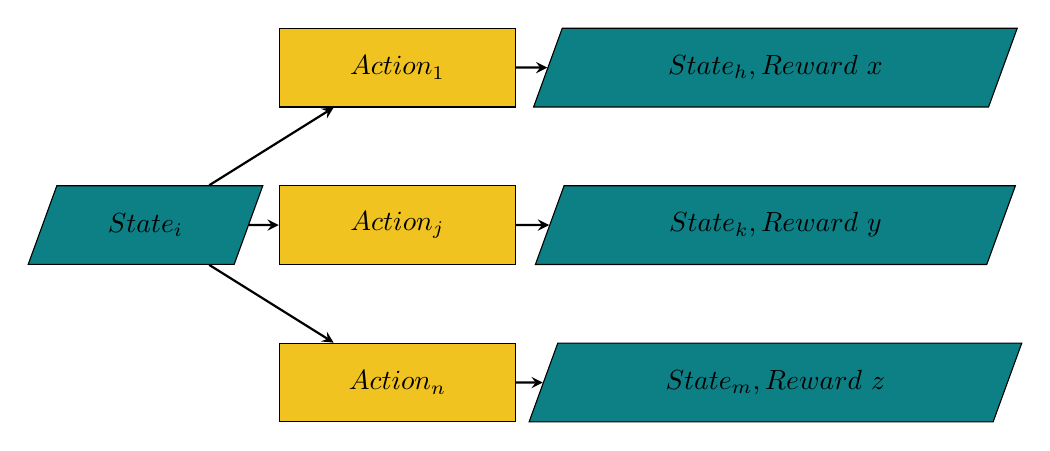
\begin{tikzpicture}[node distance=2cm]

%\node (Start) [startstop] {Start};

\node (si) [io] {$State_i$};

\node (a1) [process, right of=si, xshift=1.2cm, yshift=2cm] {$Action_1$};
\node (aj) [process, right of=si, xshift=1.2cm] {$Action_j$};
\node (an) [process, right of=si, xshift=1.2cm, yshift=-2cm] {$Action_n$};

\node (sip1) [io, right of=a1, xshift=2.8cm] {$State_{h}, Reward\ x$};
\node (sip2) [io, right of=aj, xshift=2.8cm] {$State_{k}, Reward\ y$};
\node (sip3) [io, right of=an, xshift=2.8cm] {$State_{m}, Reward\ z$};



\draw [arrow] (si) -- (a1);
\draw [arrow] (si) -- (aj);
\draw [arrow] (si) -- (an);

\draw [arrow] (a1) -- (sip1);
\draw [arrow] (aj) -- (sip2);
\draw [arrow] (an) -- (sip3);

\end{tikzpicture}
\end{frame}


\begin{frame}{The Q-Table}
\framesubtitle{The Q-Table is updated in a learning by doing approach}

Q-Updating rule introduced 1989 by Watson. Updates Q-Table according to current rewards and expected future rewards\\

$q^{new}(s_t,a_t)=(1-\alpha)q(s_t,a_t) + \alpha (r_t + \gamma \max\limits_{a} q(s_{t+1},a))$\\

$\alpha$ is learning rate, $\gamma$ is discount rate\\
$r_t$ is reward, $s_t$ is state, $a_t$ is action\\
\begin{table}

\begin{tabular}{lllll}
	\multicolumn{4}{c}{Actions}\\
	\multirow{4}{*}{States}		& $q_{s_1,a_1}$ & $q_{s_1,a_2}$ & $q_{s_1,a_3}$  & $q_{s_1,a_4}$\\
	& $q_{s_2,a_1}$ & $q_{s_2,a_2}$ & $q_{s_2,a_3}$  & $q_{s_2,a_4}$\\
	& $q_{s_3,a_1}$ & $q_{s_3,a_2}$ & $q_{s_3,a_3}$  & $q_{s_3,a_4}$\\
	& $q_{s_4,a_1}$ & $q_{s_4,a_2}$ & $q_{s_4,a_3}$  & $q_{s_4,a_4}$\\
\end{tabular}
\end{table}

\end{frame}

\begin{frame}{Choosing an action}

\begin{itemize}
\item If random number $<\epsilon$, take a random action (exploration)
\item Otherwise, take the action with the highest $q$-value (exploitation)
\end{itemize}

\end{frame}

\begin{frame}{Examples}

\begin{itemize}
	\item A simple game on the blackboard
	\item Navigate a maze with q-learning
\end{itemize}

\end{frame}



{
	\usebackgroundtemplate{
		\begin{picture}(320,315)
		\hspace{6.9cm}
		
\includegraphics[width=0.7\linewidth]{../figures/refuel_logo_with_text.png}
		\end{picture}
	}
	
	
	\begin{frame}
	\frametitle{Thank you!}
	\begin{block}{
			For slides and source-code, check \textbf{https://github.com/joph/Machine-Learning-Workshop}\\
			mail: johannes.schmidt@boku.ac.at\\
			
		}
	\end{block}
	
	\vspace{2.5 cm}
	
	
\end{frame}

}



\end{document} 